\chapter{Timer Family}\label{ch:sw-timer}

Libre-V offers three different timer options: \begin{enumerate}
  \item \hyperref[sec:sw-basic-timer]{Basic Timer}
  \item General Purpose Timer 
  \item Advanced Timer/PWM
\end{enumerate}

These timer variants differ in their functionality. The feature set increases in the order listed above. All modules are memory mapped APB peripherals.

\section{Basic Timer (BTimer)}\label{sec:sw-basic-timer}

The BTimer module is the ``APB timer'' from the PULP platform. It is a free-running 32-bit up-counter with a programmable clock prescaler and a compare register, and it raises two physical\footnote{By physical we mean that the interrupts are exposed as output ports as opposed to updating registers. These interrupts are made software-readable by connecting it to interrupt ports of the cores either pico or rocket.} interrupts: a counter \emph{overflow} and a \emph{compare match}. 

Note that the BTimer module can instantiate several \texttt{timer} cores behind an internal APB address mux (selected by \texttt{PADDR}). See \autoref{fig:timer-schematic} for a high level view of the module.
\begin{figure}[htbp]
  \centering
  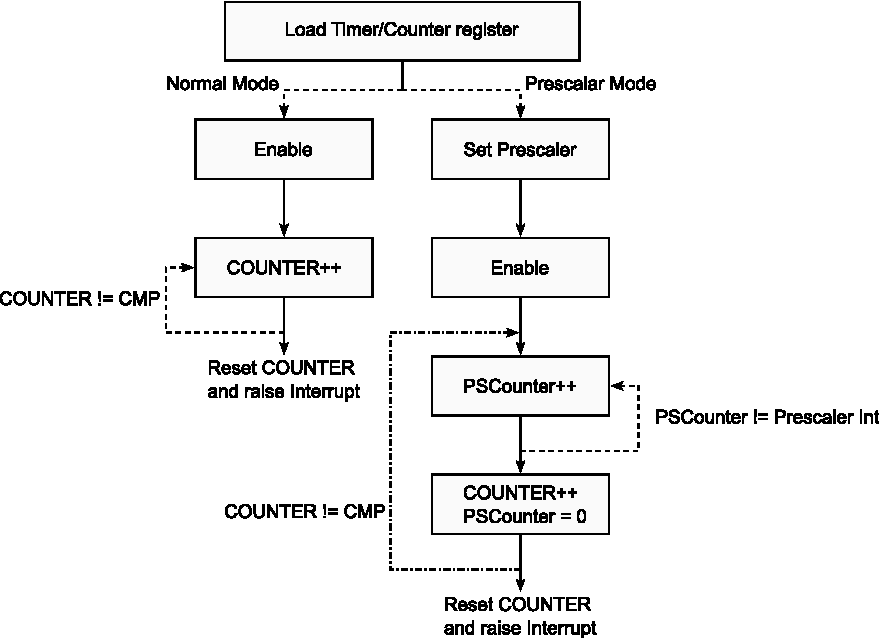
\includegraphics[width=0.85\textwidth]{figures/btimer_flow.pdf}
  \caption{Btimer control flow}
  \label{fig:btimer-flow}
\end{figure}

The Btimer core exposes three 32-bit registers. They are byte-addressed on 4-byte boundaries; the
register index is taken from APB address bits \texttt{PADDR[3:2]}:
\[
\texttt{byte\_offset} = \texttt{PADDR[3:2]} \times 4
\]

\begin{docnote}
  The base address of a Btimer can be found in the generated software library file(s) as these depend on the user-specific configuration. Offsets in this document are relative to the timer instance base.
\end{docnote}

\section*{Using the Btimer}

Figure~\autoref{fig:btimer-flow} illustrates the control flow of the Btimer module. 

\subsection{Counting and the Prescaler}

When \textbf{CTRL.EN} is set, the counter advances at a rate governed by the 3-bit prescaler field
\textbf{CTRL.PSC}. A free-running \emph{cycle counter} counts input clock cycles from \texttt{0} up
to the prescaler value and then wraps:
\begin{itemize}[nosep]
  \item \textbf{PSC = 0} (normal mode): the counter increments on every clock cycle.
  \item \textbf{PSC $\neq$ 0} (prescaled mode): the counter increments once every
        $(\mathrm{PSC}+1)$ clock cycles.
\end{itemize}
So the effective counting rate is $f_{\mathrm{clk}} / (\mathrm{PSC}+1)$.

\subsection{Compare, Overflow, and Auto-reset}

The counter is compared against the \textbf{CMP} register on each tick:
\begin{itemize}[nosep]
  \item \textbf{Compare match}: when \texttt{CMP} $\neq 0$ and the counter equals \texttt{CMP}, the
        compare-match interrupt (\texttt{irq\_o[1]}) is asserted and the counter is reset to
        \texttt{0}. A \texttt{CMP} value of \texttt{0} disables the compare function.
  \item \textbf{Overflow}: when the counter reaches \texttt{0xFFFF\_FFFF} and the next tick occurs,
        the overflow interrupt (\texttt{irq\_o[0]}) is asserted and the counter wraps to \texttt{0}.
\end{itemize}
Both interrupts are single-cycle pulses generated combinationally on the tick. In addition,
\emph{writing} the \texttt{CMP} register resets the counter to \texttt{0}, which makes it easy to
start a fresh timed interval. This gives a straightforward periodic-tick usage: program a prescaler
and a compare value, enable the timer, and take a compare-match interrupt every
$(\mathrm{CMP}+1)\times(\mathrm{PSC}+1)$ clock cycles.

\subsection{Register Descriptions}
The following section describes the TIMER registers in the numerical order of address offset.

\regtitle{0}{Timer Counter Register (TIMER)}

\regmeta{SoC-defined}{0x000}{0x00}{RW}{Free-running count. Auto-resets on match/overflow/CMP write.}

\begin{register}{H}{Timer Counter Register (TIMER)}{}

  \regfield{COUNT}{32}{0}{{00000000000000000000000000000000}}
  \reglabel{Reset}

  \regfieldvalue{COUNT}{32}{0}{{RW}}
  \reglabel{Type}

\end{register}

\textbf{Functional Description.}

Offset \texttt{0x000} holds the current 32-bit counter value. A read returns the instantaneous
count. A write preloads the counter, allowing software to start from an arbitrary value. When the
timer is enabled the hardware advances this register at the prescaled rate, and clears it to
\texttt{0} on a compare match, on overflow, or when the \textbf{CMP} register is written.

\begin{regmap}
31:0 & COUNT & RW & 0 &
Current timer count. Readable at any time; a write preloads the counter. Advances at
$f_{\mathrm{clk}}/(\mathrm{PSC}+1)$ while \textbf{CTRL.EN} = 1. \\
\end{regmap}

\regtitle{1}{Timer Control Register (CTRL)}

\regmeta{SoC-defined}{0x004}{0x00}{RW}{Only EN (bit 0) and PSC (bits 5:3) are functional.}

\begin{register}{H}{Timer Control Register (CTRL)}{}

  \regfield[gray!20]{Reserved}{26}{6}{{0}}
  \regfield{PSC}{3}{3}{000}
  \regfield[gray!20]{Reserved}{2}{1}{{0}}
  \regfield{EN}{1}{0}{0}
  \reglabel{Reset}

  \regfieldvalue[gray!20]{Reserved}{26}{6}{{RW}}
  \regfieldvalue{PSC}{3}{3}{{RW}}
  \regfieldvalue[gray!20]{Reserved}{2}{1}{{RW}}
  \regfieldvalue{EN}{1}{0}{{RW}}
  \reglabel{Type}

\end{register}

\textbf{Functional Description.}

The Control Register enables the counter and sets the prescaler. The full 32-bit word is stored, so
the reserved bits are writable and read back their last written value, but they have no effect on
operation.

\begin{regmap}
31:6 & reserved & RW & 0 &
Reserved. Stored but have no effect. \\
5:3  & PSC      & RW & 0 &
Prescaler. The counter increments once every $(\mathrm{PSC}+1)$ clock cycles. \texttt{PSC = 0}
selects normal mode (increment every cycle). \\
2:1  & reserved & RW & 0 &
Reserved. Stored but have no effect. \\
0    & EN       & RW & 0 &
Enable. When 1, the counter runs; when 0, the counter is frozen at its current value. \\
\end{regmap}

\regtitle{2}{Timer Compare Register (CMP)}

\regmeta{SoC-defined}{0x008}{0x00}{RW}{Writing CMP resets the counter to 0. CMP = 0 disables compare.}

\begin{register}{H}{Timer Compare Register (CMP)}{}

  \regfield{CMP}{32}{0}{{0}}
  \reglabel{Reset}

  \regfieldvalue{CMP}{32}{0}{{RW}}
  \reglabel{Type}

\end{register}

\textbf{Functional Description.}

Offset \texttt{0x008} holds the 32-bit compare value. When the counter reaches this value (and the
value is non-zero), the compare-match interrupt \texttt{irq\_o[1]} is asserted and the counter is
reset to \texttt{0}, producing a periodic tick of period $(\mathrm{CMP}+1)\times(\mathrm{PSC}+1)$ clock
cycles. Writing this register also immediately resets the counter to \texttt{0}, so software should
program \textbf{CMP} before starting the count. A value of \texttt{0} disables the compare path,
leaving only the overflow interrupt active.

\begin{regmap}
31:0 & CMP & RW & 0 &
Compare value. On \texttt{COUNT == CMP} (with \texttt{CMP} $\neq 0$) the compare-match interrupt
fires and the counter clears. Writing this field also clears the counter. \texttt{CMP = 0}
disables the compare match. \\
\end{regmap}

\subsection{Interrupts}

The timer core drives a 2-bit interrupt output \texttt{irq\_o[1:0]}:

\begin{tabular}{@{}cll@{}}
\toprule
\textbf{Bit} & \textbf{Name} & \textbf{Condition} \\
\midrule
0 & Overflow      & Counter wraps from \texttt{0xFFFF\_FFFF}. \\
1 & Compare match & Counter equals a non-zero \texttt{CMP}. \\
\bottomrule
\end{tabular}

\subsection{Address Map Summary}

\begin{tabular}{@{}lll@{}}
\toprule
\textbf{Offset} & \textbf{Register} & \textbf{Access} \\
\midrule
0x000 & TIMER (counter) & RW \\
0x004 & CTRL (control)  & RW \\
0x008 & CMP (compare)   & RW \\
\bottomrule
\end{tabular}

% \section{APB Advanced Timer} 

% Sourced from OpenHW Group's Core-V-MCU\footnote{\href{https://docs.openhwgroup.org/projects/core-v-mcu/doc-src/ip-blocks/apb_adv_timer.html}{https://docs.openhwgroup.org/projects/core-v-mcu/doc-src/ip-blocks/apb\_adv\_timer.html}}, the APB Advanced Timer (AAT) is capable of generating PWM for external devices. A single AAT module contains 4 independent, configurable/programmable 16-bit timer modules. 

% \subsection*{Features} 
% \begin{itemize}
%   \item Dual clock source design (APB interface clock + independent clock).
%   \item Multiple input sources: PWM/GPIO.
%   \item Configurable input trigger modes for each timer
%   \item Configurable prescaler for each timer 
%   \item Configurable counting mode for each timer 
%   \item Four comparators for each timer. 
%   \item Configurable channel comparator threshold and comparator operation for each comparator. 
%   \item Four configurable output events 4-bit PWM output for each timer. 
%   \item Configurable clock gating of each timer
% \end{itemize}

% \subsection{Block architecture} 

% Each of the four 16-bit timer is organized as an input stage, prescaler, up-down counter, and comparators. To enable MMIO integration, each of these includes a set of control registers. 

% Each of the APB Timer can generate 4-bit PWM signals (we can have 4 such 4-bit PWMs due to indepedence of all the timer modules). A 4-bit output event can be generated by configuring the \texttt{EVENT\_CFG} register. 

% \begin{figure}[htbp]
%   \centering
%   
\includegraphics[width=0.95\textwidth]{figures/tmp/apb_adv_timer_block_diagram.png}
%   \caption{APB Advanced Timer block diagram.}
%   \label{fig:apb-adv-timer-blk}
% \end{figure}

% \begin{figure}[htbp]
%   \centering
%   
\includegraphics[width=0.95\textwidth]{figures/tmp/apb_adv_timer_diagram_1.png}
%   \caption{APB Timer (child module) block diagram.}
%   \label{fig:apb-adv-timer-blk-tmp}
% \end{figure}

% \subsubsection{Timer Module}


% % \section{Overview}


% % \subsection{Source Files}

% % \begin{tabular}{@{}ll@{}}
% % \toprule
% % \textbf{File} & \textbf{Role} \\
% % \midrule
% % \texttt{apb\_timer/src/timer.sv}          & Single timer core: counter, prescaler, compare, IRQs \\
% % \texttt{apb\_timer/src/apb\_timer.sv}     & Multi-timer APB wrapper with internal address mux \\
% % \texttt{apb\_timer/src/apb\_timer\_wrap.sv} & Struct-to-flat APB wrapper around one \texttt{timer} core \\
% % \texttt{axi\_timer/axi\_timer.sv}         & NoC-side AXI4 $\rightarrow$ APB adapter chain \\
% % \bottomrule
% % \end{tabular}

% % \newpage


% \newpage